\documentclass{article}
\usepackage{setspace}
\usepackage{listings}
\usepackage{color}
\usepackage{amsmath}
\usepackage{amssymb}
\usepackage{amsthm}
\usepackage{graphicx} 
\usepackage{float} 
\usepackage{fancyhdr}                                
\usepackage{lastpage}                                           
\usepackage{layout}   
\usepackage{subfigure} 
\definecolor{codegreen}{rgb}{0,0.6,0}
\definecolor{codegray}{rgb}{0.5,0.5,0.5}
\definecolor{codepurple}{rgb}{0.58,0,0.82}
\definecolor{backcolour}{rgb}{0.95,0.95,0.92}

\lstdefinestyle{mystyle}{
    backgroundcolor=\color{backcolour},   
    commentstyle=\color{codegreen},
    keywordstyle=\color{magenta},
    numberstyle=\tiny\color{codegray},
    stringstyle=\color{codepurple},
    basicstyle=\footnotesize,
    breakatwhitespace=false,         
    breaklines=true,                 
    captionpos=b,                    
    keepspaces=true,                 
    numbers=left,                    
    numbersep=5pt,                  
    showspaces=false,                
    showstringspaces=false,
    showtabs=false,                  
    tabsize=2
}
\pagestyle{fancy}  
\lhead{ZHANG HUAKANG}
\chead{Assignment 5} 
\rhead{DB92760} 
\renewcommand{\baselinestretch}{1.05}
\title{Assignment 5 of CISC 2002}
\author{ZHANG Huakang/DB92760}

\begin{document}
    \maketitle
    \section{}
        \subsection{}
            \paragraph{
                \lstinputlisting[language=Matlab,style=mystyle,caption=Code ]{code/Assignment_5_1_1.m}
                \lstinputlisting[language=Matlab,style=mystyle,caption=Output ]{code/Assignment_5_1_1output}
            }
        \subsection{}
            \paragraph{
                \begin{equation*}
                    \begin{split}
                        P(x)=&\frac{(x-x_1)(x-x_2)(x-x_3)(x-x_4)(x-x_5)}{(x_0-x_1)(x_0-x_2)(x_0-x_3)(x_0-x_4)(x_0-x_5)}y_0\\
                            &+\frac{(x-x_0)(x-x_2)(x-x_3)(x-x_4)(x-x_5)}{(x_1-x_0)(x_1-x_2)(x_1-x_3)(x_1-x_4)(x_1-x_5)}y_1\\
                            &+\frac{(x-x_0)(x-x_1)(x-x_3)(x-x_4)(x-x_5)}{(x_2-x_0)(x_2-x_1)(x_2-x_3)(x_2-x_4)(x_2-x_5)}y_2\\
                            &+\frac{(x-x_0)(x-x_1)(x-x_2)(x-x_4)(x-x_5)}{(x_3-x_0)(x_3-x_1)(x_3-x_2)(x_3-x_4)(x_3-x_5)}y_3\\
                            &+\frac{(x-x_0)(x-x_1)(x-x_2)(x-x_3)(x-x_5)}{(x_4-x_0)(x_4-x_1)(x_4-x_2)(x_4-x_3)(x_4-x_5)}y_4\\
                            &+\frac{(x-x_0)(x-x_1)(x-x_2)(x-x_3)(x-x_4)}{(x_5-x_0)(x_5-x_1)(x_5-x_2)(x_5-x_3)(x_5-x_4)}y_5\\
                            =&\frac{(x-4)(x-6)(x-8)(x-10)(x-12)}{(2-4)(2-6)(2-8)(2-10)(2-12)}2\\
                            &+\frac{(x-2)(x-6)(x-8)(x-10)(x-12)}{(4-2)(4-6)(4-8)(4-10)(4-12)}4\\
                            &+\frac{(x-2)(x-4)(x-8)(x-10)(x-12)}{(6-2)(6-4)(6-8)(6-10)(6-x12)}4\\
                            &+\frac{(x-2)(x-4)(x-6)(x-10)(x-x12)}{(8-2)(8-4)(8-6)(8-10)(8-12)}5\\
                            &+\frac{(x-2)(x-4)(x-6)(x-8)(x-12)}{(10-2)(10-4)(10-6)(10-8)(10-12)}5\\
                            &+\frac{(x-2)(x-4)(x-6)(x-8)(x-10)}{(12-2)(12-4)(12-6)(12-8)(12-10)}7\\
                    \end{split}
                \end{equation*}
            }
        \subsection{}
            \paragraph{
                \begin{equation*}
                    A=
                    \begin{bmatrix}
                        1&0&0&0&0&0\\
                        1&2&0&0&0&0\\
                        1&4&8&0&0&0\\
                        1&6&24&48&0&0\\
                        1&8&48&192&384&0\\
                        1&10&80&480&1920&3840\\
                    \end{bmatrix}
                    ,
                    \vec{y}=
                    \begin{bmatrix}
                        2\\
                        4\\
                        4\\
                        5\\
                        5\\
                        7\\    
                    \end{bmatrix}
                \end{equation*}
                \begin{equation*}
                    \begin{split}
                        A\vec{c}=\vec{y}\\
                    \end{split}
                \end{equation*}
                \begin{equation*}
                    \begin{split}
                        \begin{bmatrix}
                            1&0&0&0&0&0\\
                            1&2&0&0&0&0\\
                            1&4&8&0&0&0\\
                            1&6&24&48&0&0\\
                            1&8&48&192&384&0\\
                            1&10&80&480&1920&3840\\
                        \end{bmatrix}
                        \begin{bmatrix}
                            c_0\\c_1\\c_2\\c_3\\c_4\\c_5\\
                        \end{bmatrix}=&
                        \begin{bmatrix}
                            2\\
                            4\\
                            4\\
                            5\\
                            5\\
                            7\\    
                        \end{bmatrix}\\
                    \end{split}
                \end{equation*}
                We can get the augmented matrix
                \begin{equation*}
                    \begin{split}
                        \begin{bmatrix}
                            1&0&0&0&0&0&2\\
                            1&2&0&0&0&0&4\\
                            1&4&8&0&0&0&4\\
                            1&6&24&48&0&0&5\\
                            1&8&48&192&384&0&5\\
                            1&10&80&480&1920&3840&7\\
                        \end{bmatrix}
                    \end{split}
                \end{equation*}
                $R_n=R_n-R_1,n\in[2,6]$
                \begin{equation*}
                    \begin{split}
                        \begin{bmatrix}
                            1&0&0&0&0&0&2\\
                            0&2&0&0&0&0&2\\
                            0&4&8&0&0&0&2\\
                            0&6&24&48&0&0&3\\
                            0&8&48&192&384&0&3\\
                            0&10&80&480&1920&3840&5\\
                        \end{bmatrix}
                    \end{split}
                \end{equation*}
                $R_n=R_n-kR_2,n\in[3,6],k\in \mathbb{R}$
                \begin{equation*}
                    \begin{split}
                        \begin{bmatrix}
                            1&0&0&0&0&0&2\\
                            0&2&0&0&0&0&2\\
                            0&0&8&0&0&0&-2\\
                            0&0&24&48&0&0&-3\\
                            0&0&48&192&384&0&-5\\
                            0&0&80&480&1920&3840&-5\\
                        \end{bmatrix}
                    \end{split}
                \end{equation*}
                $R_n=R_n-kR_3,n\in[4,6],k\in \mathbb{R}$
                \begin{equation*}
                    \begin{split}
                        \begin{bmatrix}
                            1&0&0&0&0&0&2\\
                            0&2&0&0&0&0&2\\
                            0&0&8&0&0&0&-2\\
                            0&0&0&48&0&0&3\\
                            0&0&0&192&384&0&7\\
                            0&0&0&480&1920&3840&15\\
                        \end{bmatrix}
                    \end{split}
                \end{equation*}
                $R_n=R_n-kR_4,n\in[5,6],k\in \mathbb{R}$
                \begin{equation*}
                    \begin{split}
                        \begin{bmatrix}
                            1&0&0&0&0&0&2\\
                            0&2&0&0&0&0&2\\
                            0&0&8&0&0&0&-2\\
                            0&0&0&48&0&0&3\\
                            0&0&0&0&384&0&-5\\
                            0&0&0&0&1920&3840&-15\\
                        \end{bmatrix}
                    \end{split}
                \end{equation*}
                $R_6=R_6-5R_5$
                \begin{equation*}
                    \begin{split}
                        \begin{bmatrix}
                            1&0&0&0&0&0&2\\
                            0&2&0&0&0&0&2\\
                            0&0&8&0&0&0&-2\\
                            0&0&0&48&0&0&3\\
                            0&0&0&0&384&0&-5\\
                            0&0&0&0&0&3840&10\\
                        \end{bmatrix}
                    \end{split}
                \end{equation*}
                We can get
                \begin{equation*}
                    \begin{split}
                        \begin{bmatrix}
                            1&0&0&0&0&0&2\\
                            0&1&0&0&0&0&1\\
                            0&0&1&0&0&0&-\frac{1}{4}\\
                            0&0&0&1&0&0&\frac{1}{16}\\
                            0&0&0&0&1&0&-\frac{5}{384}\\
                            0&0&0&0&0&1&\frac{1}{384}\\
                        \end{bmatrix}
                    \end{split}
                \end{equation*}
                \begin{equation*}
                    \vec{c}=
                    \begin{bmatrix}
                        2\\1\\-\frac{1}{4}\\\frac{1}{16}\\-\frac{4}{384}\\\frac{1}{384}\\
                    \end{bmatrix}
                \end{equation*}
            }
        \subsection{}
            \lstinputlisting[language=Matlab,style=mystyle,caption=Code ]{code/Assignment_5_1_2.m}
            \begin{figure}[H] 
                \centering 
                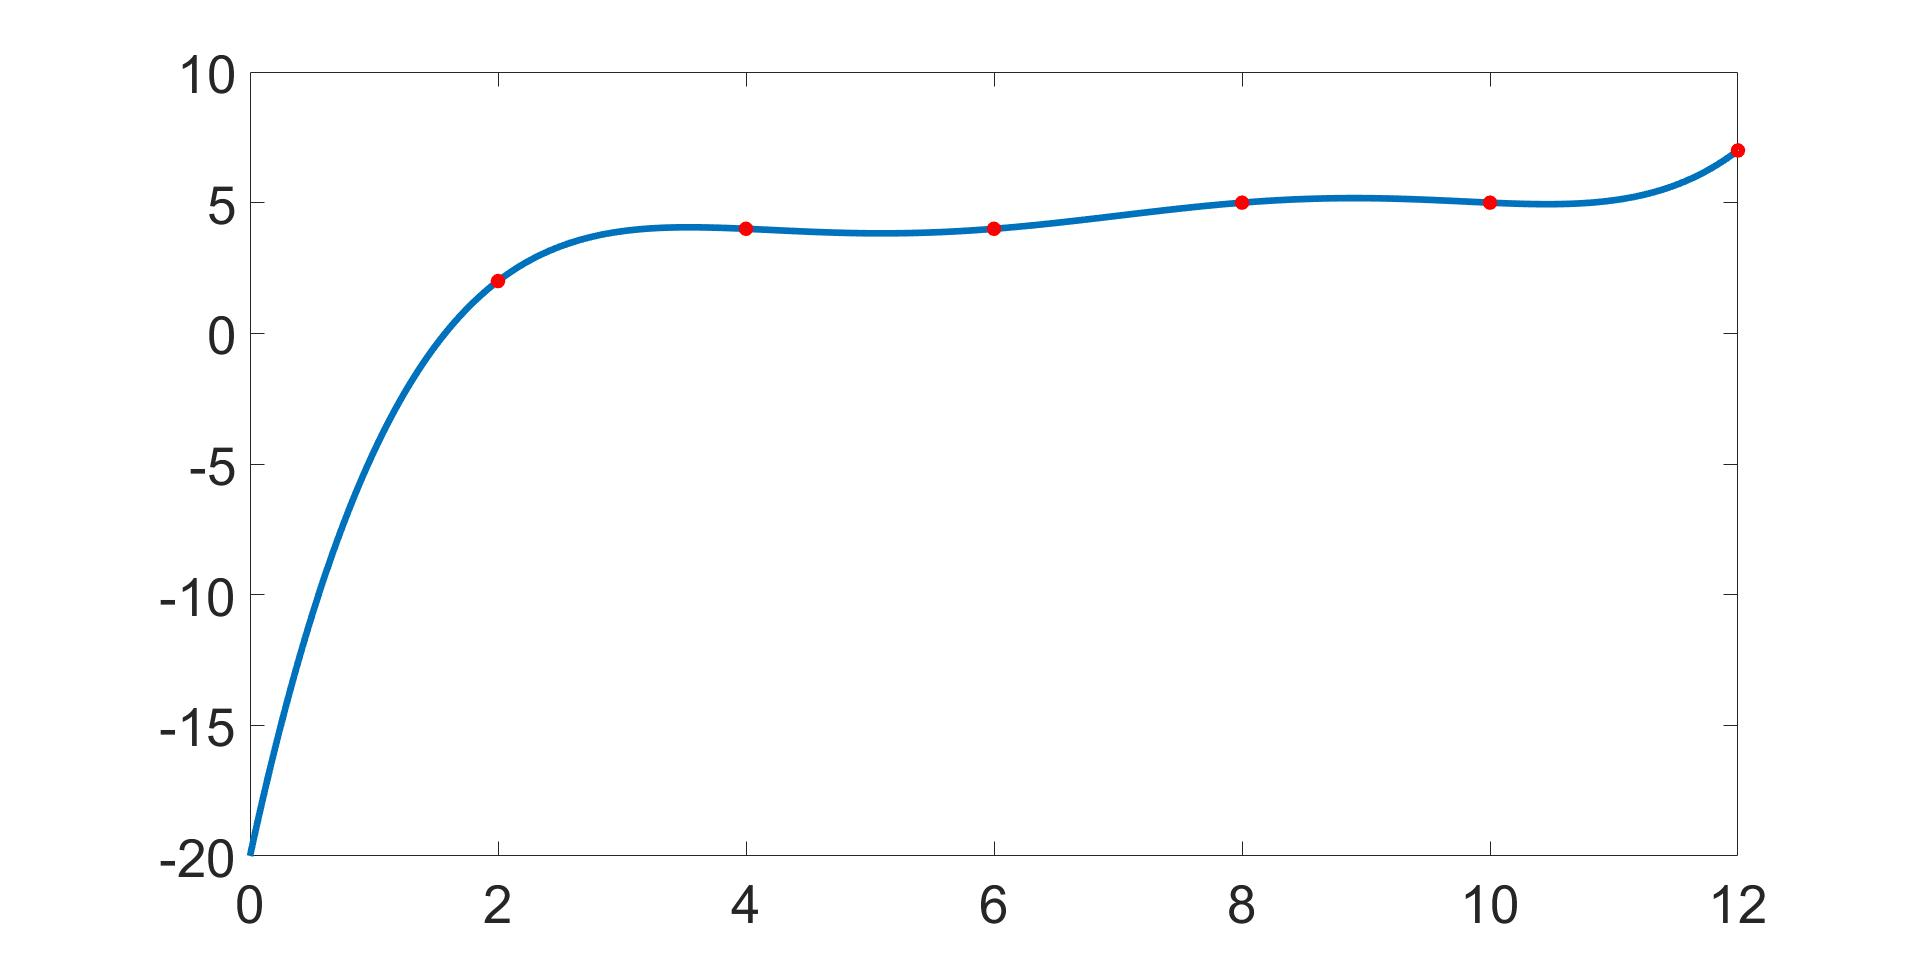
\includegraphics[width=0.9\textwidth]{img/Assignement_5_1.jpg}
                \caption{Figure} 
            \end{figure}
            
    \section{}
        \subsection{}
            \paragraph{
                \lstinputlisting[language=Matlab,style=mystyle,caption=Code ]{code/Assignment_5_2_1.m}
                \lstinputlisting[language=Matlab,style=mystyle,caption=Output ]{code/Assignment_5_2_1output}
            }
        \subsection{}
            \begin{figure}[H] 
                \centering 
                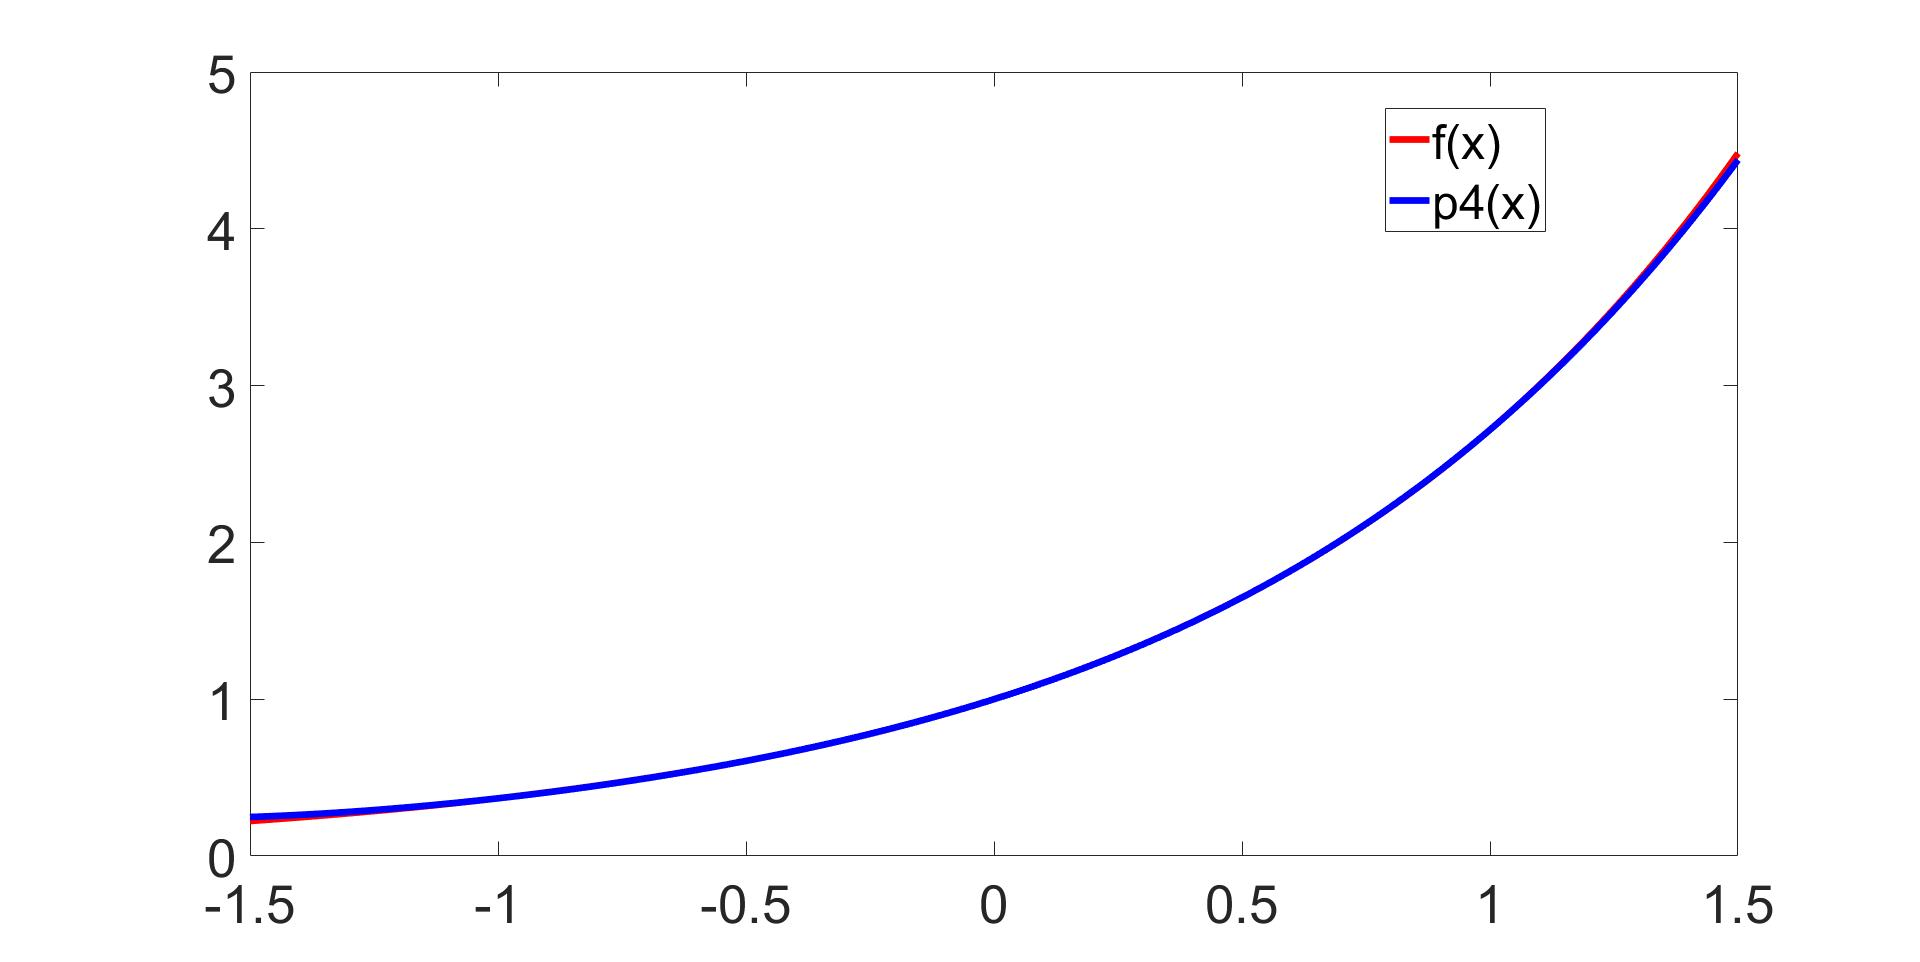
\includegraphics[width=0.9\textwidth]{img/Assignement_5_2.jpg}
                \caption{Figure} 
            \end{figure}
    \section{}
        \subsection{}
        \paragraph{
            \lstinputlisting[language=Matlab,style=mystyle,caption=Code ]{code/Assignment_5_3_1.m}
            \lstinputlisting[language=Matlab,style=mystyle,caption=Output ]{code/Assignment_5_3_1output}
        }
        \subsection{}
            \begin{figure}[H] 
                \centering 
                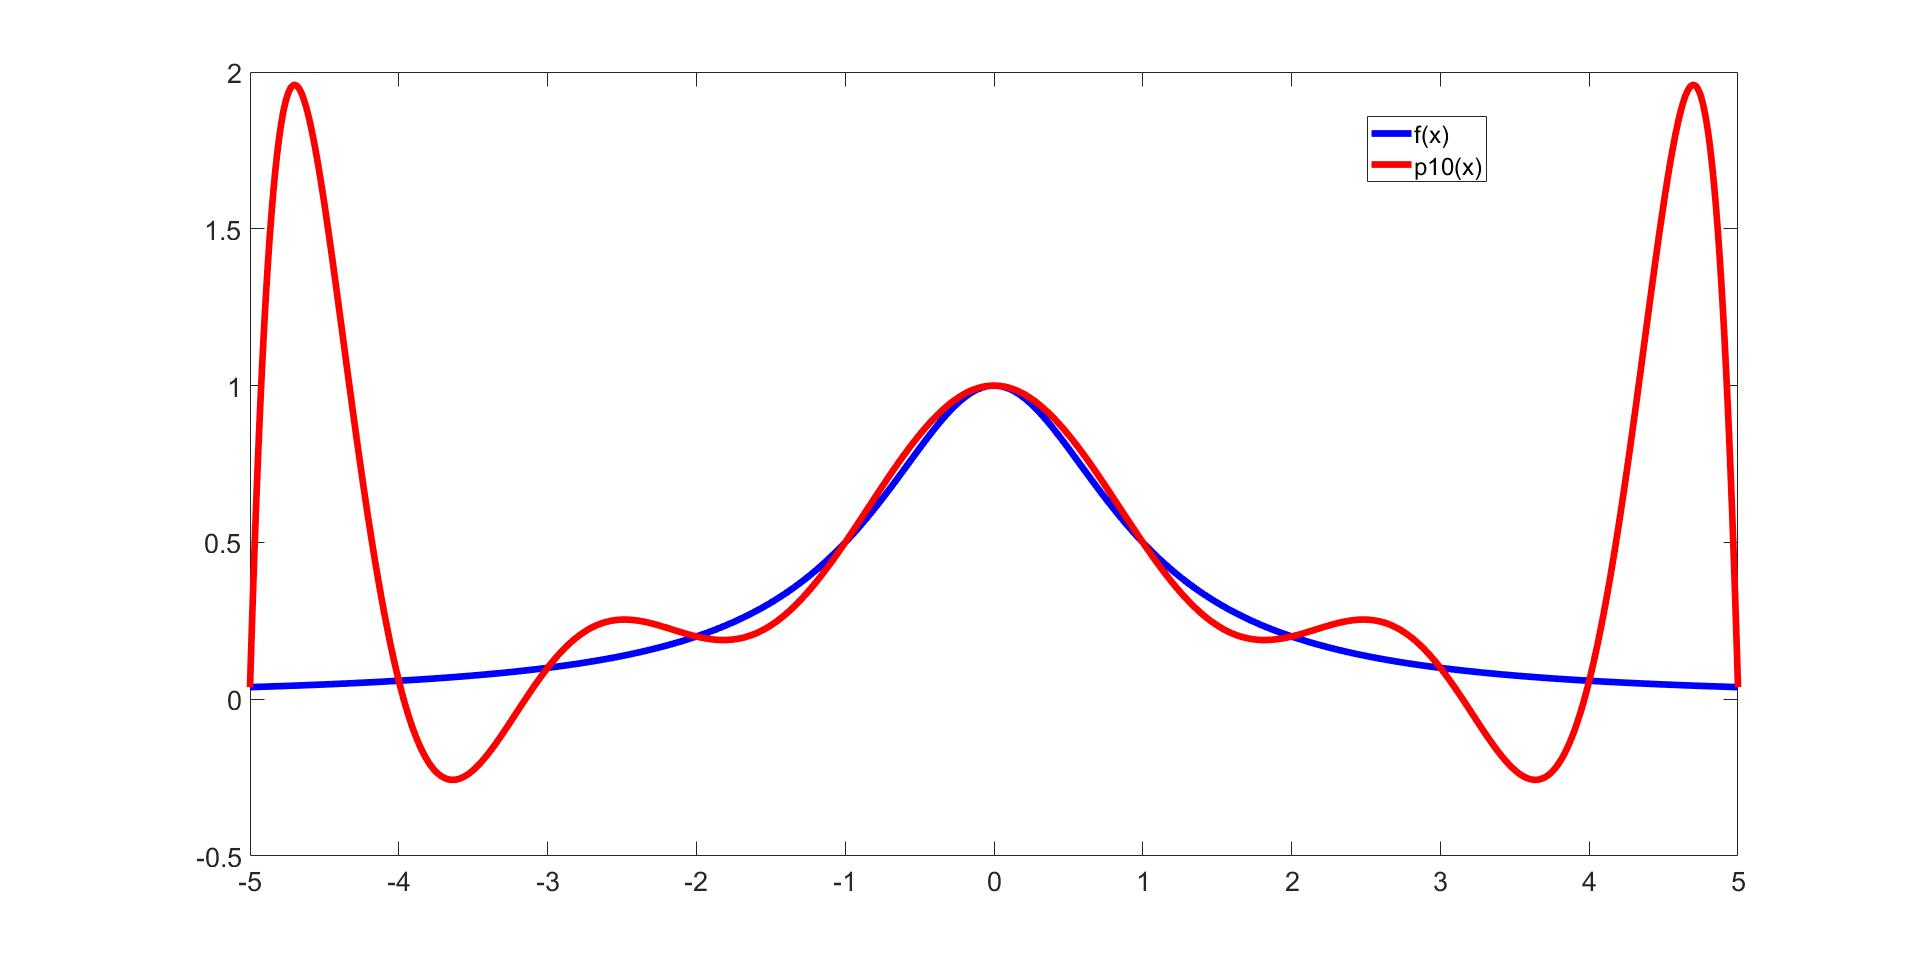
\includegraphics[width=0.9\textwidth]{img/Assignement_5_3.jpg}
                \caption{Figure} 
            \end{figure}
    \section{}
        \subsection{}
            \paragraph{
                \lstinputlisting[language=Matlab,style=mystyle,caption=Code ]{code/Assignment_5_4_1.m}
                \lstinputlisting[language=Matlab,style=mystyle,caption=Output ]{code/Assignment_5_4_1output}
            }
        \subsection{}
            \lstinputlisting[language=Matlab,style=mystyle,caption=Code ]{code/Assignment_5_4_2.m}
            \begin{figure}[H] 
                \centering 
                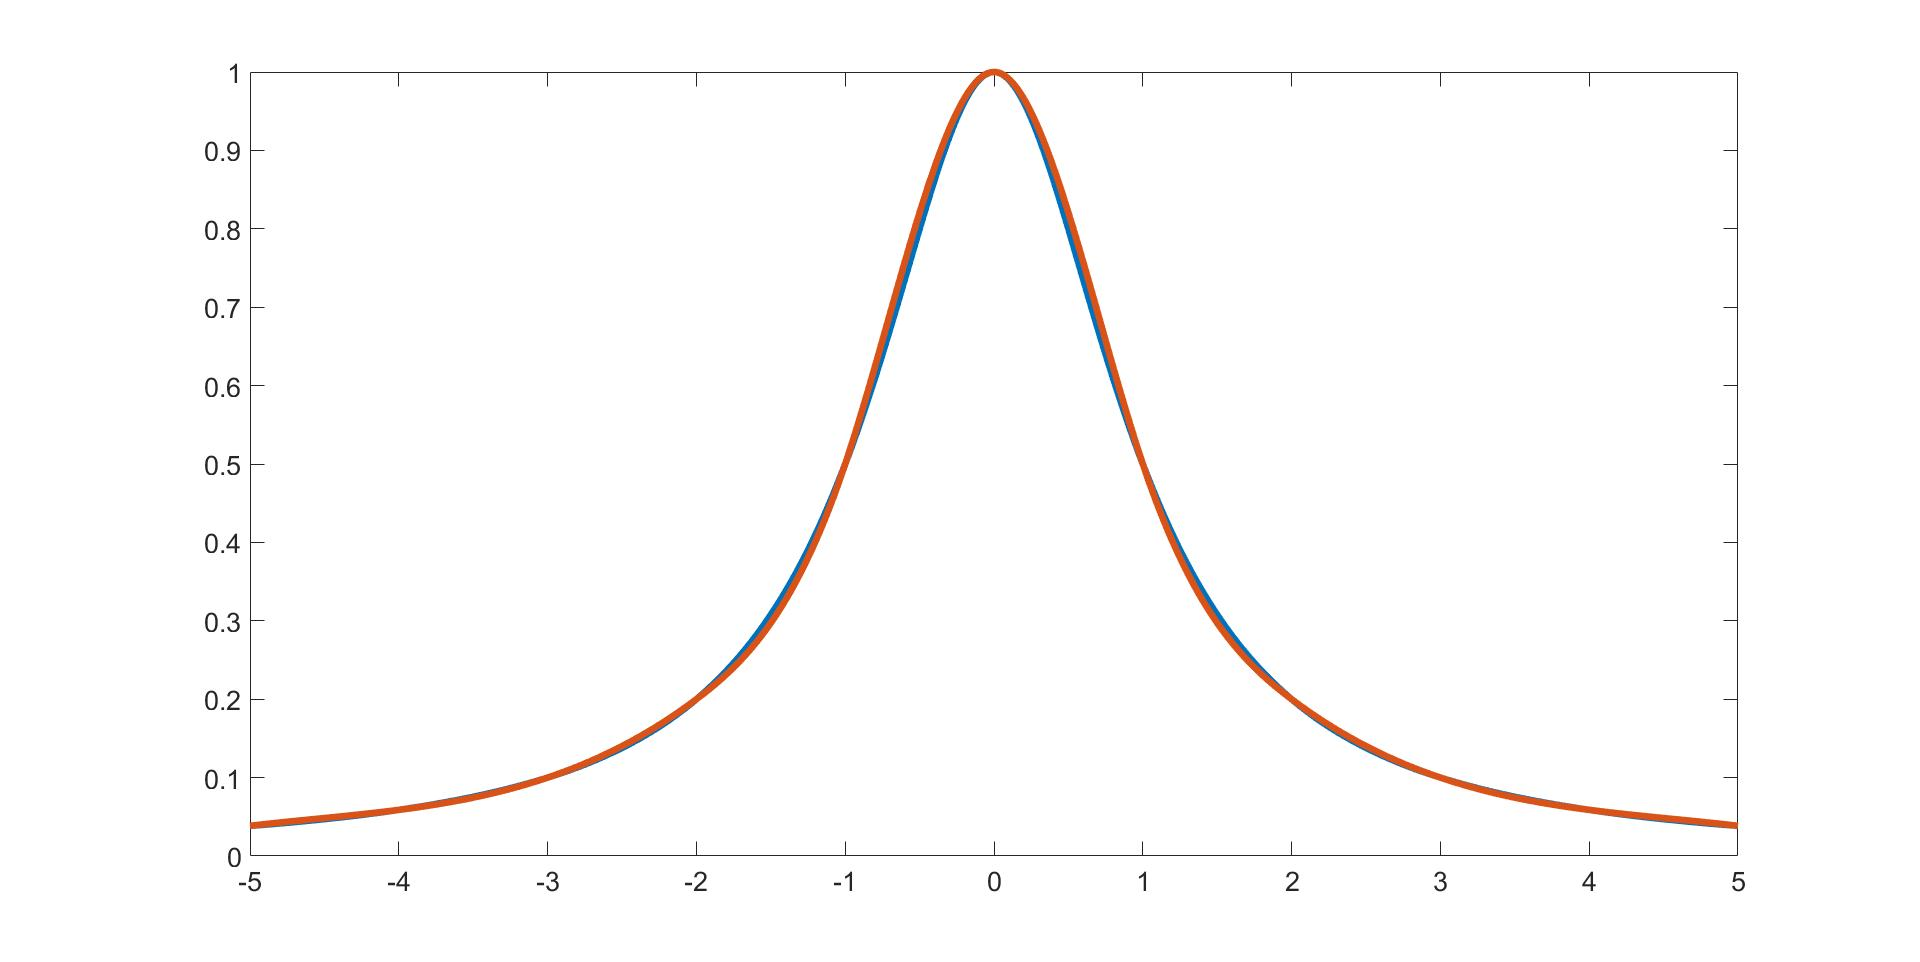
\includegraphics[width=0.9\textwidth]{img/Assignement_5_4.jpg}
                \caption{Figure} 
            \end{figure}
        \subsection{}
            \paragraph{
                Let 
                $$g_i(x)=a_i(x-x_i)^3+b_i(x-x_i)^2+c_i(x-x_i)+d_i$$
                where
                \begin{equation*}
                    \begin{split}
                        g_i(x_i)=&y_i\\
                        g_i(x_{i+1})=&y_{i+1}\\
                        g_i'(x_{i+1})=&g_{i+1}'(x_{i+1})\\
                        g_i''(x_{i+1})=&g_{i+1}''(x_{i+1})\\
                    \end{split}
                \end{equation*}
                We get
                \begin{equation*}
                    \begin{split}
                        g_0(-5)=&\frac{1}{26}\\
                        g_0(0)=&1\\
                        g'_0(0)=&g'_1(0)\\
                        g''_0(0)=&g''_1(0)\\
                        g_1(0)=&0\\
                        g_1(5)=&\frac{1}{26}\\
                        g_0'(-5)=&0\\
                        g_1'(5)=&0\\
                    \end{split}
                \end{equation*}
                Find the solution
                \begin{equation*}
                    \begin{split}
                        d_0=&\frac{1}{26}\\
                        d_1=&1\\
                        c_0=&0\\
                        b_1=&0\\
                        a_0=&-\frac{1}{260}\\
                        b_0=&\frac{3}{52}\\
                        c_1=&\frac{15}{52}\\
                        a_1=&-\frac{1}{100}\\
                    \end{split}
                \end{equation*}
                $$g(x)=-\frac{1}{260}(x+5)^3+\frac{1}{26}$$
                when $x\in[-5,0]$
                $$g(x)=-\frac{1}{100}x^3+\frac{15}{52}x+1$$
                when $x\in(0,5]$
            }
    \section{}
    \paragraph{
        \lstinputlisting[language=Matlab,style=mystyle,caption=Code ]{code/Assignment_5_5_1.m}
        \lstinputlisting[language=Matlab,style=mystyle,caption=Output ]{code/Assignment_5_5_1output}
    }
\end{document}  